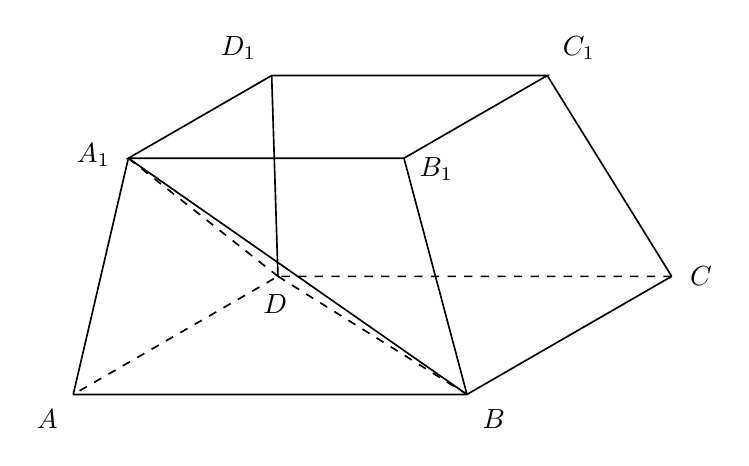
\begin{tikzpicture}[x=1cm,y=1cm,font=\normalsize,line width=.6pt]
\coordinate (A) at (0,0);
\coordinate (B) at (5,0);
\coordinate (C) at (7.6000000000,1.5000000000);
\coordinate (D) at (2.6000000000,1.5000000000);
\coordinate (Aone) at (0.7000000000,3.0000000000);
\coordinate (Bone) at (4.2000000000,3.0000000000);
\coordinate (Cone) at (6.0200000000,4.0500000000);
\coordinate (Done) at (2.5200000000,4.0500000000);
% bottom face
\draw[solid] (A) -- (B) -- (C);
\draw[dashed] (C) -- (D) -- (A);
\draw[dashed] (D) -- (B);
% top face
\draw[solid] (Aone) -- (Bone) -- (Cone) -- (Done) -- cycle;
% lateral edges
\draw[solid] (A)--(Aone);
\draw[solid] (B) -- (Bone);
\draw[solid] (C) -- (Cone);
\draw[solid] (D)--(Done);
% interior explored edges
\draw[solid] (Aone) -- (B);

% labels offset to avoid touching strokes
\node[below left,xshift=-2pt,yshift=-2pt] at (A) {$A$};
\node[below right,xshift=2pt,yshift=-2pt] at (B) {$B$};
\node[right,xshift=3pt] at (C) {$C$};
\node[below,xshift=-1pt,yshift=-3pt] at (D) {$D$};
\node[left,xshift=-3pt,yshift=1pt] at (Aone) {$A_{1}$};
\node[right,xshift=2pt,yshift=-4pt] at (Bone) {$B_{1}$};
\node[above right,xshift=2pt,yshift=2pt] at (Cone) {$C_{1}$};
\node[above left,xshift=-2pt,yshift=2pt] at (Done) {$D_{1}$};
\draw[dashed] (Aone)--(D);
\end{tikzpicture}
